\documentclass[12pt,a4paper]{article}

\usepackage{amssymb}
\usepackage{amsmath}
% These packages give access to frequently used mathematical
% symbols, such as blackboard bold for real and complex numbers.
%\usepackage{graphicx}

%\usepackage[dvips]{graphicx} % For postscript figures under latex.

\usepackage[pdftex]{graphicx} % For jpg etc figures under pdflatex.

\linespread{1.6}
% gives double-spacing

\numberwithin{equation}{section}

\tolerance = 10000
% this allows wider interword spaces without complaints




\setlength{\oddsidemargin}{8mm}
\setlength{\evensidemargin}{8mm}
\setlength{\topmargin}{-5mm}

\setlength{\textwidth}{145mm}
\setlength{\textheight}{220mm}




\begin{document}


\vglue 1cm




\begin{center}
{\Huge
\bf
Characterisation of
\\
\vspace{5mm}
Multipartite Entanglement}

\vskip 1cm

{\Large
G14PJA
\\
Mathematics 3rd Year Project
\\
Autumn
2012/2013}
\\

\vskip 5mm

{\large
\it
School of Mathematical Sciences
\\
University of Nottingham
}

\vskip 15mm

{\Large
\bf
Thomas MacLean}

\vskip 5mm

{\large
Supervisor: Dr.~Adesso}
% or Professor NN

{\large
Division: Mathematical Physics}
% Supervisor's Division: Pure or Applied or Statistics

{\large
Project code: GA P1}
% From Project Book.
% If the project is not from the book, delete the line.

{\large
Assessment type: Investigation}
% Review or Investigation



\vskip 5mm

{\large
January 2013}
% hand-in month and year

\end{center}

\vskip 1 cm

\noindent
{\it I~have read and understood the School and University guidelines
on plagiarism. I~confirm that this work is my own, apart from the
acknowledged references.}






\newpage

\vglue 1cm

\begin{center}
{\bf Abstract}
\end{center}

\vskip 1cm

\begin{center}
\begin{minipage}[c]{5in}
We investigate whether the monogamy which can be found in three qubit systems holds in mixed-state systems of four qubits. We construct a relevant system and find, from the definitions of the tangle, that it exhibits the expected behaviour. We also show that the four qubit Werner and GHZ states exhibit this monogamy whilst finding an analytical expression for the latter.
\end{minipage}
\end{center}



\newpage

\tableofcontents

\newpage











\section{Introduction}
\label{sec:intro}

Much research has been done on measures of entanglement in recent years and quantum information theory is just one are which uses this work. Books such as \cite{NielsenChuang} have been written on the subject but there is still a lot to learn. Since the publication of a well-known paper \cite{CKW}, research has been extensive on the so-called tangle \cite{OV} \cite{LOSU}. However, whilst papers are being published on certain systems \cite{EOSU} very little is known about larger systems. This paper attempts to help in answering whether properties of the smaller systems, such as monogamy and symmetry, transfer to the larger ones.

Using the definitions of the tangle and various properties discovered by other researchers, we show that monogamy holds for a few specific quantum systems, but find it difficult to discover anything certain about the symmetry.

We start in section \ref{sec:background} with the basics of quantum information theory and definitions which will later be used. In section \ref{sec:mainSection}, the most important and relevant definitions for this paper are given, ending with a background of the previous type of work done on this subject. Section \ref{sec:fourQubits} contains the various attempts made on the problem, with a successful outcome, whilst section \ref{sec:extra} gives two more supporting examples before the work is summarised in section \ref{sec:conclusions}. Appendix \ref{app:calculations} contains some supporting material for section \ref{sec:fourQubits} and finally, appendix \ref{app:Matlab} gives the code used in section \ref{sec:fourQubits}

\newpage






\section{Background Material and Definitions}
\label{sec:background}

Before any progress could be made on the project, it was necessary to learn the fundamental concepts of quantum mechanics along with a variety of techniques from linear algebra. In this section, I introduce some of the concepts which are used later on and others which I have learned. The definitions are widely accepted as common knowledge to quantum theorists, but most of what I describe below has been learned from \cite{NielsenChuang}.

\vskip 5mm

A {\bf state space} is a Hilbert space (a complex vector space with an inner product) which is assigned to a physical system, such that the system can be described by a unit {\bf state vector} in it

\vskip 2mm

We define complex conjugation and then the transpose operation (or the other way round) as {\bf Hermitian conjugation} so we have that $A^\dagger = (A^*)^T = (A^T)^*$. We also note that $(A^\dagger)^\dagger = A$

\vskip 2mm

We denote a general state vector in an $n$-dimensional Hilbert space $\mathcal{H}_n$ by its {\bf ket vector} $|\psi\rangle$. This can be more easily understood by thinking of $|\psi\rangle$ as an $n \times 1$ column vector

\vskip 2mm

To form the {\bf bra vector} $\langle\psi|$, we can apply Hermitian conjugation to $|\psi\rangle$, so we may then think of the bra vector as a $1 \times n$ row vector. So if we had, $|\psi\rangle = \begin{pmatrix} a \\ b \\c \end{pmatrix}$, then $\langle\psi| = \begin{pmatrix} a^* & b^* & c^* \end{pmatrix}$

\vskip 2mm

{\bf Computational basis} kets in the $n$-dimensional Hilbert space are the $n$ ket vectors where, for the $i$th vector, all rows have entry $0$ except row $i$ which has entry $1$. For example, in $\mathcal{H}_2$ we have that $|0\rangle = \begin{pmatrix} 1 \\ 0 \end{pmatrix}$ and $|1\rangle = \begin{pmatrix} 0 \\ 1 \end{pmatrix}$. Naturally, these vectors are all pairwise orthogonal

\vskip 2mm

The {\bf tensor product} is a means of forming larger vector spaces from smaller ones. It gives us a way of dealing with multipartite systems of qubits effectively. Perhaps the easiest way to think of it is in matrix form where we have, for $A$ as an $m$ by $n$ matrix and $B$ as a $p$ by $q$ matrix, then $A \otimes B$ is an $mp$ by $nq$ matrix, \begin{center} $A \otimes B = \begin{pmatrix} A_{11}B & A_{12}B & \cdots & A_{1n} \\ A_{21}B & A_{22}B & \cdots & A_{2n} \\ \vdots & \vdots & \ddots & \vdots \\ A_{m1}B & A_{m2}B & \cdots & A_{mn}B \end{pmatrix}$ \end{center}
We write the tensor product of two state vectors $|\phi\rangle \in \mathcal{H}_m$ and $|\psi\rangle \in \mathcal{H}_n$ as either $|\phi\rangle|\psi\rangle$ or just $|\phi\psi\rangle \in \mathcal{H}_{m}\otimes\mathcal{H}_{n}$

\vskip 2mm

Because of the way we defined bra and ket vectors, we automatically have a definition for the outer product $|\psi\rangle\langle\phi|$ in terms of matrices. If the dimension of $|\psi\rangle$ is $n$ and the dimension of $\langle\phi|$ is $m$ then we call this outer product an {\bf operator} which takes a vector from $\mathcal{H}_m$ to $\mathcal{H}_n$. As these operators can be considered simply as matrices, they obey the usual laws of linear algebra

\vskip 2mm

The {\bf Pauli sigma matrices} are defined as follows: \begin{center} $\begin{matrix}
\sigma_0 = I = \begin{pmatrix} 1 & 0 \\ 0 & 1 \end{pmatrix} & \sigma_1 = \sigma_x = \begin{pmatrix} 0 & 1 \\ 1 & 0 \end{pmatrix} \\ \sigma_2 = \sigma_y = \begin{pmatrix} 0 & -i \\ i & 0 \end{pmatrix} & \sigma_3 = \sigma_z = \begin{pmatrix} 1 & 0 \\ 0 & -1 \end{pmatrix} \end{matrix}$ \end{center}
and as an example, here I show that the outer product representation in the computational basis as defined previously is $\sigma_y = -i|0\rangle\langle1| + i|1\rangle\langle0|$. As a check, $|0\rangle\langle1| = \begin{pmatrix} 1 \\ 0 \end{pmatrix} \begin{pmatrix} 0 & 1 \end{pmatrix} = \begin{pmatrix} 0 & 1 \\ 0 & 0 \end{pmatrix}$  and also $|1\rangle\langle0| = \begin{pmatrix} 0 \\ 1 \end{pmatrix} \begin{pmatrix} 1 & 0 \end{pmatrix} = \begin{pmatrix} 0 & 0 \\ 1 & 0 \end{pmatrix}$ and so $-i|0\rangle\langle1| + i|1\rangle\langle0| = \begin{pmatrix} 0 & -i \\ 0 & 0 \end{pmatrix} + \begin{pmatrix} 0 & 0 \\ i & 0 \end{pmatrix} = \begin{pmatrix} 0 & -i \\ i & 0 \end{pmatrix} = \sigma_y$ as required

\vskip 2mm

If a system could be in one of several quantum (orthonormal) states $\{|\psi_i\rangle\}$, each with probability $\{p_i\}$  (which sum to $1$) then we describe the system by its {\bf density matrix} $\rho = \sum_{i} p_i{|\psi_i\rangle}{\langle\psi_i|}$. These density matrices have the properties:

1) $\rho^\dagger = \rho$ so it is Hermitian

2) The trace of $\rho$ is $1$, where the {\bf trace} of $\rho$ is $tr(\rho) = \sum_{j} \langle j| \rho | j\rangle$ with ${|j\rangle}$ as an orthonormal basis set. We can see straight away that in the computational basis, this is just the sum of the elements along the leading diagonal

3) $\rho$ is positive, so all of its eigenvalues are positive

\vskip 2mm

If there is only one $\{p_i\}$ (obviously equal to $1$), so the density matrix is simply given by $\rho = |\psi\rangle\langle\psi|$ then we say that $|\psi\rangle$ is a {\bf pure state}. If there is more than one probability, then the state described by the density matrix is said to be {\bf mixed}. In matrix form, if $tr(\rho^2) = 1$ then we have a pure state, but if $tr(\rho^2) < 1$ then we are dealing with a mixed state. There are other measures, such as the {\bf Von Neumann entropy}, defined as $S(\rho) = -tr(\rho \ln(\rho))$ which gives a value of $0$ only for pure states

\vskip 2mm

The {\bf partial trace} of a density matrix in a tensored Hilbert space is the operation of reducing the state by "tracing out" one of the subsystems, leaving us with the reduced density matrix in a reduced Hilbert space. For example, $\rho_{ABC}$ is in the space $\mathcal{H}_{A}\otimes\mathcal{H}_{B}\otimes\mathcal{H}_{C}$ and if we trace out subsystem B, we have $tr_{B}(\rho_{ABC}) = \rho_{AC}$ which is now in the space $\mathcal{H}_{A}\otimes\mathcal{H}_{C}$

Using our bra and ket notation, the partial trace is an easy operation to perform and is best shown by example as below. We effectively just move the subsystem we are tracing outside of the density matrix. So if we have $\rho_{ABC} = \frac{1}{2}\left(|000\rangle\langle000| + |010\rangle\langle100| + |001\rangle\langle000| + |011\rangle\langle011| \right)$ then we have $\rho_{AB} = \frac{1}{2}\left(tr_C(\rho_{ABC}) = |00\rangle\langle00|\langle0|0\rangle + |01\rangle\langle10|\langle0|0\rangle + |00\rangle\langle00|\langle1|0\rangle + |01\rangle\langle01|\langle1|1\rangle\right) = \frac{1}{2}\left(|00\rangle\langle00| + |01\rangle\langle10| + |00\rangle\langle00| + |01\rangle\langle01|\right)$ due to orthogonality of $|0\rangle$ and $|1\rangle$

\newpage







\section{The Concurrence and the Tangle}
\label{sec:mainSection}

\subsection{Two More Important Concepts}
\label{subsec:moreDefinitions}

\subsubsection{Superposition}
\label{subsubsec:superposition}

One of the defining principles of quantum mechanics is {\bf superposition}. Whereas in classical physics a bit can be either in the state $0$ or the state $1$, in quantum mechanics, a quantum bit, or a qubit, can be in the state $|0\rangle$, the state $|1\rangle$ or a superposition of the two. So we denote this as $|\phi\rangle = a|0\rangle + b|1\rangle$, where $a,b \in \mathbb{C}$ and $|a|^2 + |b|^2 = 1$.

However, when we perform a measurement on such a system, the systems is said to collapse from its superposition to a definite state. From this comes the idea of Schr\"{o}dinger's cat \cite{SCat}: that a system is in an indefinite state, such as our superposition, until we measure it at which point we disturb the system and force it into a known state.

\vskip 2mm

\subsubsection{Entanglement}
\label{subsubsec:entanglement}

Also, one of, if not \emph{the} most noteworthy traits of quantum mechanics is the concept of {\bf entanglement}. This is why it has been appropriate to assign its discussion a whole separate section. Entanglement is the idea that two or more quantum systems can interact to become entangled so that they share some information between them. This then means that none of the systems can be (fully) described without reference to the others involved.

As an example, we consider the Bell state $|\Phi^+\rangle = \frac{1}{\sqrt{2}}(|01\rangle + |10\rangle)$. We note that if we try to reduce this pure state, we get that $tr_{A}(\Phi^+) = tr_{B}(\Phi^+) = \frac{1}{2}\mathbb{I}_{2}$ which is the maximally mixed state. So we see that the reduction does not give us a pure state, so the original state must be entangled. As it happens, this Bell state (and the 3 others) are the maximally entangled states.

The physical interpretation of this state is as follows: The state $|\Phi^+\rangle$ is in a quantum superposition of states at the start and we are unable to say anything about subsystem $A$ or $B$ separately. However, if Alice makes a measurement on system $A$, then if she finds that her measurement gives the outcome $|0\rangle$ then we know with absolute certainty that if Bob makes a measurement on system $B$, he will find the state $|1\rangle$ as the state will have collapsed into $|01\rangle$. Similarly, if Alice finds $|1\rangle$ then we know that the system will have collapsed into $|10\rangle$ and so Bob will certainly find that his measurement gives him the outcome $|0\rangle$.



\subsection{Introducing the Concurrence and the Tangle}
\label{subsec:introducing}

In this section, I follow through the start of the paper by Coffman, Kundu and Wooters \cite{CKW} and review their definitions of the tangle for a measure of entanglement between first two, then multiple qubits.

For a pair of qubits $A$ and $B$, we define the "spin-flipped" density matrix to be $\tilde{\rho}_{AB} = (\sigma_y\otimes\sigma_y)\rho_{AB}^*(\sigma_y\otimes\sigma_y)$ where $\rho_{AB}$ is the original density matrix, expressed in terms of the computational basis.

Then we define the square roots of the eigenvalues (in decreasing order) of the matrix $\rho_{AB}\tilde{\rho}_{AB}$ as $\lambda_1$, $\lambda_2$, $\lambda_3$ and $\lambda_4$. Then the concurrence of the matrix $\rho_{AB}$ is $C(\rho_{AB}) = $max$\{\lambda_1-\lambda_2-\lambda_3-\lambda_4,0\}$ and then the tangle of the matrix is $\tau(\rho_{AB}) = (C(\rho_{AB}))^2$

Also written in the paper is that if the state $\rho_{AB}$ is pure, then it can be shown that the tangle of the state is simply $\tau_{AB} = \tau(\rho_{AB}) = 4\det(\rho_A)$ where we have $\rho_A$ as the partial trace of $\rho_{AB}$ over qubit $B$


\subsection{The Three Qubit Case}
\label{subsec:threeQubits}

The next section of paper \cite{CKW} is devoted to the definition of the tangle for three qubits. For a pure state $\rho_{ABC}$, we introduce some more notation and define $\tau_{A(BC)}$ as the tangle between qubit $A$ and the pair of qubits $BC$. As described in the paper, we may consider the pair $BC$ as a single qubit as, though it is in a higher dimensional state space, it can still be fully described by just two eigenstates with non-zero eigenvalues.

For mixed states, we encounter more of a problem, in that $\tau_{A(BC)}$ is not defined due to the fact that the reduced density matrix for just qubits $BC$ may require $4$ eigenstates to describe it, so we may no longer consider the pair as a single qubit. So the authors of the paper have defined the quantity $\tau_{A(BC)}^{min}$ instead. This is done by considering all pure-state decompositions of $\rho$, so all $\{(\psi_i,p_i)\}$ such that $\rho = \sum_{i}p_i|\psi_i\rangle\langle\psi_i|$ and then taking the minimum of the average value $\langle\tau_{A(BC)}\rangle = \sum_{i}p_i\tau_{A(BC)}(\psi_i)$

After some algebra which is explained in the paper, we are given the equation $\tau_{AB} + \tau_{AC} \leq \tau_{A(BC)}$. This says that the entanglement of qubit $A$ with the pair $BC$ is an upper bound for the entanglement which $A$ has with both $B$ and $C$ separately. The difference between the two sides of the inequality is then considered to be the amount of entanglement between $A$ and the pair which does not come from entanglement with the separate qubits. This entanglement is inherently tripartite and is called the residual tangle, denoted $\tau_{ABC}$.

The rest of the paper discovers properties of the residual tangle, such that it is monogamous and symmetric, so $\tau_{ABC} \geq 0$ and that the residual tangle is (at least for $3$ qubits) invariant under permutations: we find that $\tau_{A(BC)} - \tau_{AB} - \tau_{AC} = \tau_{ABC} = \tau_{B(CA)} - \tau_{BC} - \tau_{BA}$ and the same for if we construct the residual tangle around qubit $C$.

\newpage











\section{The Four Qubit Case}
\label{sec:fourQubits}

\subsection{Problem Statement}
\label{subsec:fourStatement}

The question that this paper tries to answer is whether the same properties hold for the so-called four-tangle. We want to find whether $\tau_{ABCD} \geq 0$ for all density matrices $\rho$, so that we can say that the four tangle is {\bf monogamous}. We would also like to see if the four-tangle is {\bf symmetric} so that if we construct the four-tangle around either of the four qubits, we get the same value.

We shall start by investigating $|\psi_{pure}\rangle = a\sqrt{p}|0000\rangle + b\sqrt{p}|1110\rangle + c\sqrt{1-p}|0011\rangle + d\sqrt{1-p}|0101\rangle + f\sqrt{1-p}|1001\rangle$ as one of the reduced density matrices \ref{app:purification} has already had a full analysis and this could be useful.


\subsection{Monogamy Attempts (Chronologically)}
\label{subsec:fourMonogamy}

\subsubsection{Starting Point}
\label{subsubsec:fourStart}

We start with the monogamy of the four-tangle:

$\tau_{A(BCD)} = \tau_{AB} + \tau_{AC} + \tau_{AD} + \tau_{ABC} + \tau_{ABD} + \tau_{ACD} + \tau_{ABCD}$

\noindent and then by using the definition in \cite{CKW} that $\tau_{ABC} = \tau_{A(BC)} - \tau_{AB} - \tau_{AC}$ and rearranging, we get that

$\tau_{ABCD} = \tau_{A(BCD)} - \tau_{A(BC)} - \tau_{A(BD)} - \tau_{A(CD)} + \tau_{AB} + \tau_{AC} + \tau_{AD}$

\vskip 2mm

As we know that $\tau_{A(BCD)}$ for a pure state is just $4det(\rho_{A})$, we find $\rho_{A}$ using the method described in \ref{app:redDensMat} and find that $\rho_{A} = (p|a|^2 + (1-p)|c|^2 + (1-p)|d|^2)|0\rangle\langle0| + (p|b|^2 + (1-p)|f|^2)|1\rangle\langle1|$. From this, it is obvious that $4det(\rho_{A}) = 4p^2|a|^2|b|^2 + 4p(1-p)(|a|^2|f|^2+|b|^2|c|^2+|b|^2|d|^2) + 4(1-p)^2(|c|^2|f|^2+|d|^2|f|^2)$

\vskip 2mm

Next, we consider the pairwise tangles as these are calculable from the reduced density matrices

\newpage

\subsubsection{The Pairwise Tangles}
\label{subsubsec:fourPairwise}

Here, we shall calculate $\tau_{AC}$ as an example, but a similar method is used to calculate the other pairwise tangles and the results shall simply be given.

$\rho_{AC} = \begin{pmatrix} p|a|^2+|d|^2(1-p) & 0 & 0 & 0 \\ 0 & |c|^2(1-p) & fc^*(1-p) & 0 \\ 0 & cf^*(1-p) & |f|^2(1-p) & 0 \\ 0 & 0 & 0 & p|b|^2 \end{pmatrix}$

To generalise the method (so that it may be used for $\tau_{AB}$ as well as making the algebra clearer) we rename the elements of the matrix:

\begin{center}
$\rho_{AC} = \begin{pmatrix} \alpha & 0 & 0 & 0 \\ 0 & \beta & \epsilon & 0 \\ 0 & \epsilon^* & \gamma & 0 \\ 0 & 0 & 0 & \delta \end{pmatrix}$ and from \ref{app:spinFlip} we have $\tilde{\rho}_{AC} = \begin{pmatrix} \delta^* & 0 & 0 & 0 \\ 0 & \gamma^* & \epsilon & 0 \\ 0 & \epsilon^* & \beta^* & 0 \\ 0 & 0 & 0 & \alpha^* \end{pmatrix}$
\end{center}

Then we note that $\alpha = \alpha^*$, $\beta = \beta^*$, $\gamma = \gamma^*$, $\delta = \delta^*$ and $|\epsilon|^2 = \beta\gamma$ so that

\begin{center}
$\rho_{AC}\tilde{\rho}_{AC} = \begin{pmatrix} \alpha\delta & 0 & 0 & 0 \\ 0 & 2\beta\gamma & 2\beta\epsilon & 0 \\ 0 & 2\gamma\epsilon^* & 2\beta\gamma & 0 \\ 0 & 0 & 0 & \alpha\delta \end{pmatrix}$
\end{center}

To find the eigenvalues, we use $\det(\rho_{AC}\tilde{\rho}_{AC} - I\lambda) = 0$

$(\alpha\delta - \lambda)[(2\beta\gamma - \lambda)(2\beta\gamma - \lambda)(\alpha\delta - \lambda) - 2\beta\epsilon(2\gamma\epsilon^*(\alpha\delta - \lambda))] = 0$

$(\alpha\delta - \lambda)^2[(2\beta\gamma - \lambda)^2 - 4\beta\gamma|\epsilon|^2] = 0$ and then as $|\epsilon|^2 = \beta\gamma$

$(\alpha\delta - \lambda)^2[\lambda^2 - 4\beta\gamma\lambda] = 0$

$\lambda(\alpha\delta - \lambda)^2(\lambda - 4\beta\gamma) = 0$

Giving the eigenvalues as $\lambda = 0$, $\lambda = \alpha\delta$ (twice) and $\lambda = 4\beta\gamma$

From here, we can create conditions from the definition of the concurrence/tangle and then give the tangle of the matrix exactly.

$C(\rho_{AC}) = $max$\{\lambda_1-\lambda_2-\lambda_3-\lambda_4,0\}$ where the $\lambda$ are the square roots of $\rho_{AC}\tilde{\rho}_{AC}$ in decreasing order. As we only have two unique, nonzero eigenvalues, we have three cases:

\noindent 1) $\alpha\delta > 4\beta\gamma$

$C(\rho_{AC}) = $max$\{\sqrt{\alpha\delta} - \sqrt{\alpha\delta} - 2\sqrt{\beta\gamma} - 0,0\} = 0$

and so naturally $\tau_{AC} = 0$ as well

\noindent 2) $\alpha\delta = 4\beta\gamma$

$C(\rho_{AC}) = $max$\{\sqrt{\alpha\delta} - \sqrt{\alpha\delta} - \sqrt{\alpha\delta} - 0,0\} = 0$

and again $\tau_{AC} = 0$

\noindent 3) $\alpha\delta < 4\beta\gamma$

$C(\rho_{AC}) = $max$\{2\sqrt{\beta\gamma} - \sqrt{\alpha\delta} - \sqrt{\alpha\delta} - 0,0\} = $max$\{2\sqrt{\beta\gamma} - 2\sqrt{\alpha\delta},0\}$

We note that this condition can be furthered to $\alpha\delta < \beta\gamma$

So we can put this all together and say the tangle is $0$ unless $\alpha\delta < \beta\gamma$ in which case $\tau_{AC} = 4\beta\gamma - 8\sqrt{\alpha\beta\gamma\delta} + 4\alpha\delta$

Then in terms of the original problem, we have that the tangle is $0$ unless $p^2|a|^2|b|^2 + p(1-p)|b|^2|d|^2 < (1-p)^2|c|^2|f|^2$ in which case we have a result that $\tau_{AC} = 4(1-p)^2|c|^2|f|^2 - 8(1-p)|b||c||f|\sqrt{p^2|a|^2 + p(1-p)|d|^2} +4p^2|a|^2|b|^2 + 4p(1-p)|b|^2|d|^2$

\vskip 2mm

The other cases are fairly similar and the results are given below:

\vskip 2mm

For $\tau_{AB}$, the tangle is $0$ unless $p^2|a|^2|b|^2 + p(1-p)|b|^2|c|^2 < (1-p)^2|d|^2|f|^2$ in which case $\tau_{AB} = 4(1-p)^2|d|^2|f|^2 - 8(1-p)|b||d||f|\sqrt{p^2|a|^2 + p(1-p)|c|^2} +4p^2|a|^2|b|^2 + 4p(1-p)|b|^2|c|^2$

\vskip 2mm

For $\tau_{AD}$, the tangle is $0$ unless $|b|^2(|c|^2 + |d|^2) < |a|^2|f|^2$ in which case $\tau_{AD} = 4p(1-p)|a|^2|f|^2 - 8p(1-p)|a||b||f|\sqrt{|c|^2 + |d|^2} + 4p(1-p)|b|^2|c|^2 + 4p(1-p)|b|^2|d|^2$

\vskip 2mm

So we now have only to find the tripartite tangles

\newpage

\subsubsection{The Tripartite Tangle - Approach 1}
\label{subsubsec:fourTripartite1}

One of the first approaches attempted was using the inequality from \cite{CKW} which says $\tau_{AB} + \tau_{AC} \leq \tau_{A(BC)}$. This can also be written as an equality, as is done in the paper as well: $\tau_{AB} + \tau_{AC} + \tau_{ABC} = \tau_{A(BC)}$

We start with $\tau_{ABCD} = \tau_{A(BCD)} - \tau_{A(BC)} - \tau_{A(BD)} - \tau_{A(CD)} + \tau_{AB} + \tau_{AC} + \tau_{AD}$

\noindent By substituting all of the tripartite tangles for the other side of the equality, we get $\tau_{ABCD} = \tau_{A(BCD)} - \tau_{AB} - \tau_{AC} - \tau_{AB} - \tau_{AD} - \tau_{AC} - \tau_{AD} + \tau_{AB} + \tau_{AC} + \tau_{AD} - \tau_{ABC} - \tau_{ABD} - \tau_{ACD}$ which simplifies to $\tau_{ABCD} = \tau_{A(BCD)} - \tau_{AB} - \tau_{AC} - \tau_{AD} - \tau_{ABC} - \tau_{ABD} - \tau_{ACD}$

In \cite{CKW}, it is conjectured that $\tau_{12} + \tau_{13} + ... + \tau_{1n} \leq \tau_{1(23...n)}$ but not proved. However, there is another paper, \cite{OV} in which the above is proved. So the first part of the equation, $\tau_{A(BCD)} - (\tau_{AB} + \tau_{AC} + \tau_{AD})$ is definitely greater than or equal to $0$. Then it remains to calculate these tripartite tangles, which is difficult for mixed states, due to its construction.


\subsubsection{The Tripartite Tangle - Approach 2}
\label{subsubsec:fourTripartite2}

In \cite{EOSU}, a complete analysis is given for the three-tangle of a mixture of a generalised GHZ state and a generalised W state, so we have that the density matrix is given by $\rho = p|gGHZ_{a,b}\rangle\langle gGHZ_{a,b}| + (1-p)|gW_{c,d,f}\rangle\langle gW_{c,d,f}|$

\noindent with the generalised GHZ state: $|gGHZ_{a,b}\rangle = a|000\rangle + b|111\rangle$

\noindent and the generalised W state: $|gW_{c,d,f}\rangle = c|001\rangle + d|010\rangle + f|100\rangle$

\noindent and the conditions $|a|^2 + |b|^2 = 1$ and similarly $|c|^2 + |d|^2 + |f|^2 = 1$

The paper gives results for this state, but also mentions that some of the authors had written another paper, \cite{LOSU} which is where the methods came from. In this paper is outlined a method to calculate the three-tangle for any three qubit, rank-2 density matrices of the form $\rho = p|1\rangle\langle1| + (1-p)|2\rangle\langle2|$ where $|1\rangle$ and $|2\rangle$ are orthogonal states

This has potential to be useful for calculating the three-tangle for such parts as $\rho_{ACD}$ if they are in the right form. In density matrix form, $\rho_{ACD}$ turns out to be:

\noindent $\begin{pmatrix} p|a|^2 & 0 & 0 & \sqrt{p(1-p)}ac^* & 0 & \sqrt{p(1-p)}af^* & 0 & 0 \\ 0 & (1-p)|d|^2 & 0 & 0 & 0 & 0 & \sqrt{p(1-p)}db^* & 0 \\ 0 & 0 & 0 & 0 & 0 & 0 & 0 & 0 \\ \sqrt{p(1-p)}ca^* & 0 & 0 & (1-p)|c|^2 & 0 & (1-p)cf^* & 0 & 0 \\ 0 & 0 & 0 & 0 & 0 & 0 & 0 & 0 \\ \sqrt{p(1-p)}fa^* & 0 & 0 & (1-p)fc^* & 0 & (1-p)|f|^2 & 0 & 0 \\ 0 & \sqrt{p(1-p)}bd^* & 0 & 0 & 0 & 0 & p|b|^2 & 0 \\ 0 & 0 & 0 & 0 & 0 & 0 & 0 & 0 \end{pmatrix}$

\vskip 2mm

which is of the form $\rho_{ACD} = |1\rangle\langle1| + |2\rangle\langle2|$ where we have

\vskip 2mm

$|1\rangle = \begin{pmatrix} \sqrt{p}a^* \\ 0 \\ 0 \\ \sqrt{1-p}c^* \\ 0 \\ \sqrt{1-p}f^* \\ 0 \\ 0 \end{pmatrix}$ and $|2\rangle = \begin{pmatrix} 0 \\ \sqrt{1-p}d^* \\ 0 \\ 0 \\ 0 \\ 0 \\ \sqrt{p}b^* \\ 0 \end{pmatrix}$ which are orthogonal

\vskip 2mm

These can be rewritten in the form $\rho_{ACD} = q|3\rangle\langle3| + (1-q)|4\rangle\langle4|$ via some rescaling, where $q$ is some function of $p$, which would allow them to be analysed in a similar way to \cite{LOSU} but this was only realised at the end of the project after the answer had been found. However, this method may be useful for different types of states.

\newpage

\subsubsection{The Tripartite Tangle - An Idea}
\label{subsubsec:fourTripartiteIdea}

Further in the paper \cite{LOSU}, the authors outline an approach to find a polyhedron in the Bloch Sphere within which the three-tangle of a state is zero, but non-zero otherwise. If there do exist states which break the monogamy constraint, a possible way of finding them would be to calculate states in which $\tau_{A(BCD)} - (\tau_{AB} + \tau_{AC} + \tau_{AD}) = 0$ and where the three-tangle of any of the reduced density matrices lie outside the simplex. This non-zero three-tangle would make $\tau_{ABCD}$ negative and thus break the constraint. However, due to time constraints on this project, I have been unable to take this idea further.


\subsubsection{The Tripartite Tangle - Approach 3}
\label{subsubsec:fourTripartite3}

As all other approaches seemed not to be going anywhere, it was decided that using MATLAB to try and get some numerical results would be best. So it remained to try to write code to find the $\tau_{A(BC)}$ for mixed states. In \cite{CKW}, this is defined as the minimum average value of the tangle over all possible pure-state decompositions of the original state.

So we are trying to find the minimum of $\sum_{i}p_{i}\tau_{A(BC)}(\psi_{i})$ whilst considering all sets $\{(\psi_{i},p_{i})\}$ such that $\rho = \sum_{i}p_{i}|\psi_{i}\rangle\langle\psi_{i}|$

Naturally, this is a difficult problem computationally, due to the infinite number of ways that we can find a pure-state decomposition, along with a lack of mathematical papers on how one would go about finding any. However, there is a paper by Uhlmann \cite{U} which says that if $\rho$ is a rank($\omega$) state, then a maximum of $\omega^2$ pure states are needed for the optimal decomposition of $\rho$. As the states we are considering are rank-2 states, it suffices to find ensembles of only up to 4 pure states.

Unfortunately, even with this information, I was unable to think of a way to code a program.

\newpage

\subsection{Monogamy Solution Attempt for Specific States}
\label{subsec:fourSolution}

\subsubsection{Key Parts to Approach 4}
\label{subsubsec:keyParts}

Again in this section, we concentrate on the previously mentioned mixture of states $|\psi_{pure}\rangle = a\sqrt{p}|0000\rangle + b\sqrt{p}|1110\rangle + c\sqrt{1-p}|0011\rangle + d\sqrt{1-p}|0101\rangle + f\sqrt{1-p}|1001\rangle$ and set $\rho_{ABCD} = |\psi_{pure}\rangle\langle\psi_{pure}|$

\vskip 2mm

For the basis of this argument, the equation given in the previous section is used: $\tau_{ABCD} = \tau_{A(BCD)} - \tau_{A(BC)} - \tau_{A(BD)} - \tau_{A(CD)} + \tau_{AB} + \tau_{AC} + \tau_{AD}$

\vskip 2mm

We also need the definition $\tau_{A(BC)}^{min} = \min[\sum_{i}p_{i}\tau_{A(BC)}(\psi_{i})]$ for all sets $\{(\psi_{i},p_{i})\}$ such that $\rho = \sum_{i}p_{i}|\psi_{i}\rangle\langle\psi_{i}|$

\vskip 2mm

We recall from earlier, that $4det(\rho_{A}) = 4p^2|a|^2|b|^2 + 4p(1-p)(|a|^2|f|^2+|b|^2|c|^2+|b|^2|d|^2) + 4(1-p)^2(|c|^2|f|^2+|d|^2|f|^2)$ which is the tangle between qubit $A$ and all the others, denoted $\tau_{A(BCD)}$

Finally we recall from \ref{subsubsec:fourPairwise}:

For $\tau_{AB}$, the tangle is $0$ unless $p^2|a|^2|b|^2 + p(1-p)|b|^2|c|^2 < (1-p)^2|d|^2|f|^2$ in which case $\tau_{AB} = 4(1-p)^2|d|^2|f|^2 - 8(1-p)|b||d||f|\sqrt{p^2|a|^2 + p(1-p)|c|^2} +4p^2|a|^2|b|^2 + 4p(1-p)|b|^2|c|^2$

\vskip 2mm

For $\tau_{AC}$, the tangle is $0$ unless $p^2|a|^2|b|^2 + p(1-p)|b|^2|d|^2 < (1-p)^2|c|^2|f|^2$ in which case $\tau_{AC} = 4(1-p)^2|c|^2|f|^2 - 8(1-p)|b||c||f|\sqrt{p^2|a|^2 + p(1-p)|d|^2} +4p^2|a|^2|b|^2 + 4p(1-p)|b|^2|d|^2$

\vskip 2mm

For $\tau_{AD}$, the tangle is $0$ unless $|b|^2(|c|^2 + |d|^2) < |a|^2|f|^2$ in which case $\tau_{AD} = 4p(1-p)|a|^2|f|^2 - 8p(1-p)|a||b||f|\sqrt{|c|^2 + |d|^2} + 4p(1-p)|b|^2|c|^2 + 4p(1-p)|b|^2|d|^2$

\newpage

\subsubsection{Upper Bounds of the Reduced Density Matrices' Three-tangles}
\label{subsubsec:upperBound}

We start by considering $\rho_{ACD}$ (shown in matrix form in \ref{subsubsec:fourTripartite2} as $\rho_{ACD}^{(1)} + \rho_{ACD}^{(2)}$ where we have:

\vskip 2mm

\noindent $\rho_{ACD}^{(1)} = \begin{pmatrix} 0 & 0 & 0 & 0 & 0 & 0 & 0 & 0 \\ 0 & (1-p)|d|^2 & 0 & 0 & 0 & 0 & \sqrt{p(1-p)}db^* & 0 \\ 0 & 0 & 0 & 0 & 0 & 0 & 0 & 0 \\ 0 & 0 & 0 & 0 & 0 & 0 & 0 & 0 \\ 0 & 0 & 0 & 0 & 0 & 0 & 0 & 0 \\ 0 & 0 & 0 & 0 & 0 & 0 & 0 & 0 \\ 0 & \sqrt{p(1-p)}bd^* & 0 & 0 & 0 & 0 & p|b|^2 & 0 \\ 0 & 0 & 0 & 0 & 0 & 0 & 0 & 0 \end{pmatrix}$

\vskip 2mm

\noindent and

\vskip 2mm

$\rho_{ACD}^{(2)} = \begin{pmatrix} p|a|^2 & 0 & 0 & \sqrt{p(1-p)}ac^* & 0 & \sqrt{p(1-p)}af^* & 0 & 0 \\ 0 & 0 & 0 & 0 & 0 & 0 & 0 & 0 \\ 0 & 0 & 0 & 0 & 0 & 0 & 0 & 0 \\ \sqrt{p(1-p)}ca^* & 0 & 0 & (1-p)|c|^2 & 0 & (1-p)cf^* & 0 & 0 \\ 0 & 0 & 0 & 0 & 0 & 0 & 0 & 0 \\ \sqrt{p(1-p)}fa^* & 0 & 0 & (1-p)fc^* & 0 & (1-p)|f|^2 & 0 & 0 \\ 0 & 0 & 0 & 0 & 0 & 0 & 0 & 0 \\ 0 & 0 & 0 & 0 & 0 & 0 & 0 & 0 \end{pmatrix}$

\vskip 2mm

\noindent and we notice that both $\rho_{ACD}^{(1)}$ and $\rho_{ACD}^{(2)}$ are pure states if we factor out their trace. We also note that $tr(\rho_{ACD}^{(1)}) + tr(\rho_{ACD}^{(2)}) = p|a|^2 + p|b|^2 + (1-p)|c|^2 + (1-p)|d|^2 + (1-p)|f|^2 = 1$ from the state's definition.

So a pure-state decomposition for $\rho_{ACD}$ is $tr(\rho_{ACD}^{(1)})\hat{\rho}_{ACD}^{(1)} + tr(\rho_{ACD}^{(2)})\hat{\rho}_{ACD}^{(2)}$ where $\hat{\rho}_{ACD}^{(1)}$ is the normalised version of $\rho_{ACD}^{(1)}$. However, as our next operation is linear, we may leave the trace in and consider the un-normalised version

We may now calculate $\sum_{i}p_{i}\tau_{A(CD)}(\psi_{i})$ as we know that each pure state has a tangle of $4\det(\rho_{A})$. After reducing the density matrices, we get that $\rho_{A}^{(1)} = \begin{pmatrix} (1-p)|d|^2 & 0 \\ 0 & p|b|^2 \end{pmatrix}$ and so $4\det(\rho_{A}^{(1)}) = 4p(1-p)|b|^2|d|^2$.

Similarly, $\rho_{A}^{(2)} = \begin{pmatrix} p|a|^2 + (1-p)|c|^2 & 0 \\ 0 & p|f|^2 \end{pmatrix}$ and so we get that $4\det(\rho_{A}^{(2)}) = 4p(1-p)|a|^2|f|^2 + 4(1-p)^2|c|^2|f|^2$

So we have, but only with respect to the decomposition we have used, that $\tau_{A(CD)} = 4p(1-p)|b|^2|d|^2 + 4p(1-p)|a|^2|f|^2 + 4(1-p)^2|c|^2|f|^2$

By finding this value, we know that this is an upper bound for $\tau_{A(CD)}^{min}$

\vskip 2mm

Next we see that $\rho_{A(CD)}$ is very similar to $\rho_{A(BD)}$ (as shown below) except that the $d$ and $c$ parts are the other way round:

\vskip 2mm

\noindent $\begin{pmatrix} p|a|^2 & 0 & 0 & \sqrt{p(1-p)}ad^* & 0 & \sqrt{p(1-p)}af^* & 0 & 0 \\ 0 & (1-p)|c|^2 & 0 & 0 & 0 & 0 & \sqrt{p(1-p)}cb^* & 0 \\ 0 & 0 & 0 & 0 & 0 & 0 & 0 & 0 \\ \sqrt{p(1-p)}da^* & 0 & 0 & (1-p)|d|^2 & 0 & (1-p)df^* & 0 & 0 \\ 0 & 0 & 0 & 0 & 0 & 0 & 0 & 0 \\ \sqrt{p(1-p)}fa^* & 0 & 0 & (1-p)fd^* & 0 & (1-p)|f|^2 & 0 & 0 \\ 0 & \sqrt{p(1-p)}bc^* & 0 & 0 & 0 & 0 & p|b|^2 & 0 \\ 0 & 0 & 0 & 0 & 0 & 0 & 0 & 0 \end{pmatrix}$

\vskip 2mm

so a similar analysis can take place and we get our upper bound for $\tau_{A(BD)}^{min}$ as $\tau_{A(BD)} = 4p(1-p)|b|^2|c|^2 + 4p(1-p)|a|^2|f|^2 + 4(1-p)^2|d|^2|f|^2$

From \cite{EOSU}, we are given that the three-tangle for a generalised Werner state is $0$ and for a GHZ state, is $4|a|^2|b|^2$, so by applying the same technique as we have just done for the above, we find that our upper bound for $\tau_{A(BC)}^{min}$ is $\tau_{A(BC)} = 4p^2|a|^2|b|^2$

\newpage

\subsubsection{Putting it all Together}
\label{subsubsec:comingTogether}

Let us first consider $\tau_{A(BCD)} - (\tau_{A(BC)} + \tau_{A(BD)} + \tau_{A(CD)})$. From what we found in \ref{subsubsec:upperBound} we know that a lower bound for this would be attained when we use the individual upper bounds for each of $\tau_{A(BC)}$, $\tau_{A(BD)}$ and $\tau_{A(CD)}$. Whether it is possible to find a state with these values at the same time is irrelevant. If we somehow did so, we get that our lower bound is:

\noindent $4p^2|a|^2|b|^2 + 4p(1-p)(|a|^2|f|^2+|b|^2|c|^2+|b|^2|d|^2) + 4(1-p)^2(|c|^2|f|^2+|d|^2|f|^2) - 4p^2|a|^2|b|^2 - 4p(1-p)|b|^2|c|^2 - 4p(1-p)|a|^2|f|^2 - 4(1-p)^2|d|^2|f|^2 - 4p(1-p)|b|^2|d|^2 - 4p(1-p)|a|^2|f|^2 - 4(1-p)^2|c|^2|f|^2$ which is simply equal to $-4p(1-p)|a|^2|f|^2$

At this point, I created the code in appendix \ref{app:bipartiteCode} to check if indeed it was the case that $\tau_{AB} + \tau_{AC} + \tau_{AD} \geq 4p(1-p)|a|^2|f|^2$, though it turned out not to be true in general.


\subsection{Monogamy Solution for Specific States}
\label{subsec:actualFourSolution}

This section is actually a follow-on from the first approach in section \ref{subsubsec:fourTripartite1} and finds the tripartite tangles, whilst using the bipartite information from \ref{subsubsec:fourPairwise}.

In the paper \cite{LOSU}, the authors obtain the three-tangle of the state which is denoted $\rho_{ABC}$ here. They do this by considering the superposition of the two pure states (in actual fact, one minus the other) and use the wavefunction coefficients (as below) to get an expression before analysing it when the expression evaluates to less than zero.

$\tau_3 = 4|d_1 - 2d_2 + 4d_3|$

$d_1 = \psi_{000}^2\psi_{111}^2 + \psi_{001}^2\psi_{110}^2 + \psi_{010}^2\psi_{101}^2 + \psi_{100}^2\psi_{011}^2$

$d_2 = \psi_{000}\psi_{111}\psi_{011}\psi_{100} + \psi_{000}\psi_{111}\psi_{101}\psi_{010} + \psi_{000}\psi_{111}\psi_{110}\psi_{001} + \psi_{011}\psi_{100}\psi_{101}\psi_{010} + \psi_{011}\psi_{100}\psi_{110}\psi_{001} + \psi_{101}\psi_{010}\psi_{110}\psi_{001}$

$d_3 = \psi_{000}\psi_{110}\psi_{101}\psi_{011} + \psi_{111}\psi_{001}\psi_{010}\psi_{100}$

Then we use the pure states we have found and find that (in a more general case than in \cite{LOSU}:

$\tau_{ABC} = 4(p^2a^2b^2 + 4\sqrt{p(1-p)^3}bcdf)$ (for $p_0 < p < p_1$, with more information in \cite{EOSU}). Note that this is the only density matrix which, when analysed this way, has a negative part and so requires extra attention.

However, we must remember to normalise the two density matrices first, (whereas the one above is already normalised) and so we end up with the two formulae:

$\tau_{ABD} = 4tr(\rho_{ABD}^{(1)})tr(\rho_{ABD}^{(2)})(p(1-p)c^2b^2 + 4p(1-p)abdf)$

$\tau_{ACD} = 4tr(\rho_{ACD}^{(1)})tr(\rho_{ACD}^{(2)})(p(1-p)d^2b^2 + 4p(1-p)abcf)$

At this point, with little time remaining, I decided it would be best to test these formulae in MATLAB and the code is shown in \ref{app:fullCode}.
Below is the graphical output to demonstrate that the results showed that $0 \leq \tau_{ABCD} \leq 1$ as we were hoping for. There were a few results which were actually below zero, but this was almost certainly down to rounding errors in the calculations.

\begin{figure}[ht!]
\centering
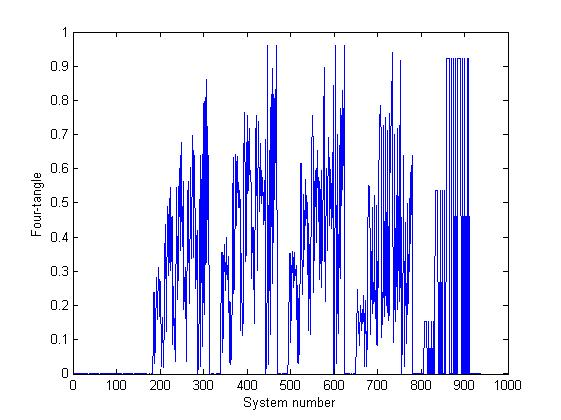
\includegraphics[width=90mm]{Figure.jpg}
\caption{States and their four-tangle}
\label{fig1}
\end{figure}

\newpage

\section{The Four-tangle of Two Other States}
\label{sec:extra}

\subsection{General GHZ State}
\label{subsec:GHZ}

For a general GHZ state with $n$ qubits, $|GHZ\rangle = a|0000\rangle + b |1111\rangle$. So we have $|GHZ\rangle\langle GHZ| = |a|^2|0000\rangle\langle0000| + ab^*|0000\rangle\langle1111| + ba^*|1111\rangle\langle0000| + |b|^2|1111\rangle\langle1111|$

As this is a pure state, we know that $\tau_{A(BCD)} = 4\det(\rho_{A})$ and as $\rho_{A} = |a|^2|0\rangle\langle0| + |b|^2|1\rangle\langle1|$ we get that $\tau_{A(BCD)} = 4|a|^2|b|^2$

For this state, $\rho_{AB} = \rho_{AC} = \rho_{AD} = |a|^2|00\rangle\langle00| + |b|^2|11\rangle\langle11|$ or in matrix form,

$\begin{pmatrix} |a|^2 & 0 & 0 & 0 \\ 0 & 0 & 0 & 0 \\ 0 & 0 & 0 & 0 \\ 0 & 0 & 0 & |b|^2 \end{pmatrix}$ with the spin-flipped version as $\begin{pmatrix} |b|^2 & 0 & 0 & 0 \\ 0 & 0 & 0 & 0 \\ 0 & 0 & 0 & 0 \\ 0 & 0 & 0 & |a|^2 \end{pmatrix}$

When multiplied together, this gives a diagonal matrix with the same two non-zero elements. Thus from our definition of the tangle for two qubits, we get that the bipartite tangles are all zero.

Again, for this state, $\rho_{ABC} = \rho_{ACD} = \rho_{ABD} = |a|^2|000\rangle\langle000| + |b|^2|111\rangle\langle111|$ which can be written as:

$|a|^2 \begin{pmatrix} 1 & 0 & 0 & 0 & 0 & 0 & 0 & 0 \\ 0 & 0 & 0 & 0 & 0 & 0 & 0 & 0 \\ 0 & 0 & 0 & 0 & 0 & 0 & 0 & 0 \\ 0 & 0 & 0 & 0 & 0 & 0 & 0 & 0 \\ 0 & 0 & 0 & 0 & 0 & 0 & 0 & 0 \\ 0 & 0 & 0 & 0 & 0 & 0 & 0 & 0 \\ 0 & 0 & 0 & 0 & 0 & 0 & 0 & 0 \\ 0 & 0 & 0 & 0 & 0 & 0 & 0 & 0 \end{pmatrix} + |b|^2 \begin{pmatrix} 0 & 0 & 0 & 0 & 0 & 0 & 0 & 0 \\ 0 & 0 & 0 & 0 & 0 & 0 & 0 & 0 \\ 0 & 0 & 0 & 0 & 0 & 0 & 0 & 0 \\ 0 & 0 & 0 & 0 & 0 & 0 & 0 & 0 \\ 0 & 0 & 0 & 0 & 0 & 0 & 0 & 0 \\ 0 & 0 & 0 & 0 & 0 & 0 & 0 & 0 \\ 0 & 0 & 0 & 0 & 0 & 0 & 0 & 0 \\ 0 & 0 & 0 & 0 & 0 & 0 & 0 & 1 \end{pmatrix}$

By noting that the two matrices are pure states, that $|a|^2 + |b|^2 = 1$ and that the reduced density matrix will be simply $\begin{pmatrix} 1 & 0 \\ 0 & 0 \end{pmatrix}$ or $\begin{pmatrix} 0 & 0 \\ 0 & 1 \end{pmatrix}$, both of which have determinant $0$, then this, in a similar way to \ref{subsubsec:upperBound} gives the tripartite tangles an upper bound of $|a|^2 \times 0 + |b|^2 \times 0 = 0$

As the tripartite tangle has been shown to be monogamous previously, $0$ is also a lower bound and thus the tripartite tangles are all $0$.

This then leaves  $\tau_{A(BCD)} = \tau_{ABCD}$ and so we finally get $\tau_{ABCD} = 4|a|^2|b|^2$


\subsection{General Werner State}
\label{subsec:Werner}

We start with $|W\rangle = a|0001\rangle + b|0010\rangle + c|0100\rangle + d|1000\rangle$ as our general Werner state. Then from \cite{CKW} we are given that $\tau_{AB} + \tau_{AC} + \tau_{AD} = \tau_{A(BCD)}$.

This being the case, the equation $\tau_{A(BCD)} = \tau_{AB} + \tau_{AC} + \tau_{AD} + \tau_{ABC} + \tau_{ABD} + \tau_{ACD} + \tau_{ABCD}$ reduces to $\tau_{ABCD} = -(\tau_{ABC} + \tau_{ABD} + \tau_{ACD})$

Then by using, $\tau_{ABC} = \tau_{A(BC)} - \tau_{AB} - \tau_{AC}$ on all three tripartite tangles, we obtain $\tau_{ABCD} = (\tau_{AB} + \tau_{AC} - \tau_{A(BC)}) + (\tau_{AC} + \tau_{AD} - \tau_{A(CD)}) + (\tau_{AB} + \tau_{AD} - \tau_{A(BD)})$

Also from \cite{CKW} we have the inequality $\tau_{AB} + \tau_{AC} \leq \tau_{A(BC)}$, and so each bracket above is less than or equal to zero.

From here, we focus on $\tau_{A(BC)}$ with the understanding that the others will be fairly similar. To find $\rho_{ABC}$, we simply form $\rho_{ABCD} = |W\rangle\langle W|$ and then take the partial trace over qubit D. This leaves us with a matrix which can again be separated in the way we did with the purification.

$\begin{pmatrix} |a|^2 & 0 & 0 & 0 & 0 & 0 & 0 & 0 \\ 0 & |b|^2 & bc^* & 0 & bd^* & 0 & 0 & 0 \\ 0 & cb^* & |c|^2 & 0 & cd^* & 0 & 0 & 0 \\ 0 & 0 & 0 & 0 & 0 & 0 & 0 & 0 \\ 0 & db^* & dc^* & 0 & |d|^2 & 0 & 0 & 0 \\ 0 & 0 & 0 & 0 & 0 & 0 & 0 & 0 \\ 0 & 0 & 0 & 0 & 0 & 0 & 0 & 0 \\ 0 & 0 & 0 & 0 & 0 & 0 & 0 & 0 \end{pmatrix}$

\vskip 2mm

The matrix is then split by taking the $|a|^2$ part as its own matrix, which is then factorised out, again leaving a matrix with a $1$ in the top left and $0$s elsewhere, having tangle $0$.

The remaining matrix involving only $b, c, d$ is also pure and reducing it gives $\begin{pmatrix} |b|^2 + |c|^2 & 0 \\ 0 & |d|^2 \end{pmatrix}$, so that $4\det(\rho_{A}) = 4|b|^2|d|^2 + 4|c|^2|d|^2$. So now we have our upper bound for $\tau_{A(BC)}$

We can figure out $\tau_{AB}, \tau_{AC}$ and similar others via the normal method. The aforementioned have values of $4|c|^2|d|^2$ and $4|b|^2|d|^2$ respectively.

\vskip 2mm

To bring everything together, we have that $\tau_{AB} + \tau_{AC} - \tau_{A(BC)} \leq 0$. We can substitute in our known values to get $4|c|^2|d|^2 + 4|b|^2|d|^2 - \tau_{A(BC)} \leq 0$. As we know that $\tau_{A(BC)} \leq 4|c|^2|d|^2 + 4|b|^2|d|^2$, the only way to satisfy all the conditions is if $\tau_{A(BC)} = 4|c|^2|d|^2 + 4|b|^2|d|^2$, so this must be the case.

The other brackets are computed the same way and so finally we have them all as $0$, giving $\tau_{ABCD} = 0 + 0 + 0 = 0$

\newpage

\section{Conclusions}
\label{sec:conclusions}

We have seen that for a purification of a mixture of a generalised GHZ state with a generalised Werner state, $|\psi_{pure}\rangle = a\sqrt{p}|0000\rangle + b\sqrt{p}|1110\rangle + c\sqrt{1-p}|0011\rangle + d\sqrt{1-p}|0101\rangle + f\sqrt{1-p}|1001\rangle$ the monogamy of the residual $4$-tangle holds, that is to say that for this state $\tau_{ABCD} \geq 0$ for all choices of $a, b, c, d, f$ such that $|a|^2 + |b|^2 = 1 = |c|^2 + |d|^2 + |f|^2$

We have also managed to show that a general GHZ state with four qubits will have a four-tangle of $4|a|^2|b|^2$, and that for four qubit systems, monogamy holds for the general Werner state as well. More specifically, it is shown that the four-tangle of a  four qubit Werner state is $0$.

Unfortunately time did not allow for an attempt to check if the four-tangle is symmetrical, though the methods used may give a clue. However, I hope that this work will push others to study the symmetry of the 4-tangle and also whether the monogamy condition holds for states other than the few studied here. Also, I hope that someone will analyse the expression for $\tau_{ABCD}$ fully, accounting for the conditions on the bipartite tangles, to check that the numerics do hold up.

\newpage

\appendix

\section{Calculations for section \ref{sec:fourQubits}}
\label{app:calculations}

\subsection{Purification of the Generalized W and GHZ States}
\label{app:purification}

In this appendix we verify that the state $|\psi_{pure}\rangle = a\sqrt{p}|0000\rangle + b\sqrt{p}|1110\rangle + c\sqrt{1-p}|0011\rangle + d\sqrt{1-p}|0101\rangle + f\sqrt{1-p}|1001\rangle$ is in fact a purification we can use by showing that by tracing out qubit D, we arrive at the mixture of generalized GHZ and Werner states we wanted.

\vskip 5mm

So we have that the density matrix is given by: $|\psi_{pure}\rangle\langle\psi_{pure}| =
 p|a|^2|0000\rangle\langle0000| + pab^*|0000\rangle\langle1110| + ac^*\sqrt{p(1-p)}|0000\rangle\langle0011| + ad^*\sqrt{p(1-p)}|0000\rangle\langle0101| + af^*\sqrt{p(1-p)}|0000\rangle\langle1001| + pba^*|1110\rangle\langle0000| + p|b|^2|1110\rangle\langle1110| + bc^*\sqrt{p(1-p)}|1110\rangle\langle0011| + bd^*\sqrt{p(1-p)}|1110\rangle\langle0101| + bf^*\sqrt{p(1-p)}|1110\rangle\langle1001| + ca^*\sqrt{p(1-p)}|0011\rangle\langle0000| + cb^*\sqrt{p(1-p)}|0011\rangle\langle1110| + |c|^2(1-p)|0011\rangle\langle0011| + cd^*(1-p)|0011\rangle\langle0101| + cf^*(1-p)|0011\rangle\langle1001| + da^*\sqrt{p(1-p)}|0101\rangle\langle0000| + db^*\sqrt{p(1-p)}|0101\rangle\langle1110| + dc^*(1-p)|0101\rangle\langle0011| + |d|^2(1-p)|0101\rangle\langle0101| + df^*(1-p)|0101\rangle\langle1001| + fa^*\sqrt{p(1-p)}|1001\rangle\langle0000| + fb^*\sqrt{p(1-p)}|1001\rangle\langle1110| + fc^*(1-p)|1001\rangle\langle0011| + fd^*(1-p)|1001\rangle\langle0101| + |f|^2(1-p)|1001\rangle\langle1001|$

\vskip 5mm

From here, we could simply note that when we trace out qubit D, all the terms with which involve a $\sqrt{p(1-p)}$ will disappear because of the way the state has been constructed and that the last qubits are different in all of these parts, but the same whenever the terms are simply multiplied by $p$ or $1-p$. Hence we will be left with just the GHZ and Werner state mixture. However, on the next page, this shall be shown explicitly.

\newpage

So we take the partial trace over qubit D:

\vskip 5mm

$tr_D(|\psi_{pure}\rangle\langle\psi_{pure}|) = p|a|^2|000\rangle\langle000|\langle0|0\rangle + pab^*|000\rangle\langle111|\langle0|0\rangle + ac^*\sqrt{p(1-p)}|000\rangle\langle001|\langle0|1\rangle + ad^*\sqrt{p(1-p)}|000\rangle\langle010|\langle0|1\rangle + af^*\sqrt{p(1-p)}|000\rangle\langle100|\langle0|1\rangle + pba^*|111\rangle\langle000|\langle0|0\rangle + p|b|^2|111\rangle\langle111|\langle0|0\rangle + bc^*\sqrt{p(1-p)}|111\rangle\langle001|\langle0|1\rangle + bd^*\sqrt{p(1-p)}|111\rangle\langle010|\langle0|1\rangle + bf^*\sqrt{p(1-p)}|111\rangle\langle100|\langle0|1\rangle + ca^*\sqrt{p(1-p)}|001\rangle\langle000|\langle1|0\rangle + cb^*\sqrt{p(1-p)}|001\rangle\langle111|\langle1|0\rangle + |c|^2(1-p)|001\rangle\langle001|\langle1|1\rangle + cd^*(1-p)|001\rangle\langle010|\langle1|1\rangle + cf^*(1-p)|001\rangle\langle100|\langle1|1\rangle + da^*\sqrt{p(1-p)}|010\rangle\langle000|\langle1|0\rangle + db^*\sqrt{p(1-p)}|010\rangle\langle111|\langle1|0\rangle + dc^*(1-p)|010\rangle\langle001|\langle1|1\rangle + |d|^2(1-p)|010\rangle\langle010|\langle1|1\rangle + df^*(1-p)|010\rangle\langle100|\langle1|1\rangle + fa^*\sqrt{p(1-p)}|100\rangle\langle000|\langle1|0\rangle + fb^*\sqrt{p(1-p)}|100\rangle\langle111|\langle1|0\rangle + fc^*(1-p)|100\rangle\langle001|\langle1|1\rangle + fd^*(1-p)|100\rangle\langle010|\langle1|1\rangle + |f|^2(1-p)|100\rangle\langle100|\langle1|1\rangle$

\vskip 5mm

And then by noting that $\langle0|1\rangle = \langle1|0\rangle = 0$ and $\langle0|0\rangle = \langle1|1\rangle = 1$ we can simplify to:

\vskip 5mm

$tr_D(|\psi_{pure}\rangle\langle\psi_{pure}|) =
p|a|^2|000\rangle\langle000| + pab^*|000\rangle\langle111| + pba^*|111\rangle\langle000| + p|b|^2|111\rangle\langle111| + |c|^2(1-p)|001\rangle\langle001| + cd^*(1-p)|001\rangle\langle010| + cf^*(1-p)|001\rangle\langle100| + dc^*(1-p)|010\rangle\langle001| + |d|^2(1-p)|010\rangle\langle010| + df^*(1-p)|010\rangle\langle100| + fc^*(1-p)|100\rangle\langle001| + fd^*(1-p)|100\rangle\langle010| + |f|^2(1-p)|100\rangle\langle100|$

\vskip 5mm

Which, when written as a state vector, we can straight away see is what we were hoping for, which was $|\Psi\rangle = p|\psi\rangle + (1-p)|\phi\rangle$ where we have defined the ket $|\psi\rangle = a|000\rangle + b|111\rangle$ as a generalized GHZ state and $|\phi\rangle = c|001\rangle + b|010\rangle + c|100\rangle$ as a generalized Werner state

\newpage

\subsection{Finding the Reduced Density Matrices}
\label{app:redDensMat}

In this section, we demonstrate how the partial trace operation is performed on $\rho_{ABCD}$ to give us $\rho_{AC}$. This method is also used to find $\rho_{A}$, $\rho_{AB}$, $\rho_{AD}$, $\rho_{ABD}$ and $\rho_{ACD}$ (with $\rho_{ABC}$ already found in the first appendix) but these are not shown.

\vskip 5mm

We start again with $\rho_{ABCD}$ and note that instead of tracing out qubits B and D separately, we may trace them both out at the same time and then use the facts that $|00\rangle\langle00| = |01\rangle\langle01| = |10\rangle\langle10| = |11\rangle\langle11| = 1$ whereas all other combinations are equal to $0$. For example, $|00\rangle\langle10| = |01\rangle\langle10| = |00\rangle\langle11| = 0$

\vskip 5mm

So $tr_{BD}(|\psi_{pure}\rangle\langle\psi_{pure}|) =
p|a|^2|00\rangle\langle00|\langle00|00\rangle + pab^*|00\rangle\langle11|\langle00|10\rangle + ac^*\sqrt{p(1-p)}|00\rangle\langle01|\langle00|01\rangle + ad^*\sqrt{p(1-p)}|00\rangle\langle00|\langle00|11\rangle + af^*\sqrt{p(1-p)}|00\rangle\langle10|\langle00|01\rangle + pba^*|11\rangle\langle00|\langle10|00\rangle + p|b|^2|11\rangle\langle11|\langle10|10\rangle + bc^*\sqrt{p(1-p)}|11\rangle\langle01|\langle10|01\rangle + bd^*\sqrt{p(1-p)}|11\rangle\langle00|\langle10|11\rangle + bf^*\sqrt{p(1-p)}|11\rangle\langle10|\langle10|01\rangle + ca^*\sqrt{p(1-p)}|01\rangle\langle00|\langle01|00\rangle + cb^*\sqrt{p(1-p)}|01\rangle\langle11|\langle01|10\rangle + |c|^2(1-p)|01\rangle\langle01|\langle01|01\rangle + cd^*(1-p)|01\rangle\langle00|\langle01|11\rangle + cf^*(1-p)|01\rangle\langle10|\langle01|01\rangle + da^*\sqrt{p(1-p)}|010\rangle\langle00|\langle11|00\rangle + db^*\sqrt{p(1-p)}|00\rangle\langle111|\langle11|10\rangle + dc^*(1-p)|00\rangle\langle01|\langle11|01\rangle + |d|^2(1-p)|00\rangle\langle00|\langle11|11\rangle + df^*(1-p)|00\rangle\langle10|\langle11|01\rangle + fa^*\sqrt{p(1-p)}|10\rangle\langle00|\langle01|00\rangle + fb^*\sqrt{p(1-p)}|10\rangle\langle11|\langle01|10\rangle + fc^*(1-p)|10\rangle\langle01|\langle01|01\rangle + fd^*(1-p)|10\rangle\langle00|\langle01|11\rangle + |f|^2(1-p)|10\rangle\langle10|\langle01|01\rangle$

\vskip 5mm

And we get that $\rho_{AC} = p|a|^2|00\rangle\langle00| + |d|^2(1-p)|00\rangle\langle00| + |c|^2(1-p)|01\rangle\langle01| + |f|^2(1-p)|10\rangle\langle10| + p|b|^2|11\rangle\langle11| + cf^*(1-p)|01\rangle\langle10| + fc^*(1-p)|10\rangle\langle01|$




\newpage

\subsection{Effect of Spin-Flipping a Matrix}
\label{app:spinFlip}

Here, we take a general $4 \times 4$ matrix and spin-slip it. From the definition, $\tilde{\rho}_{ab} = (\sigma_y\otimes\sigma_y)\rho_{ab}^*(\sigma_y\otimes\sigma_y)$

So we start with $\rho_{ab} = \begin{pmatrix} a & b & c & d \\ e & f & g & h \\ i & j & k & l \\ m & n & p & q \end{pmatrix}$ and $\sigma_y\otimes\sigma_y = \begin{pmatrix} 0 & 0 & 0 & -1 \\ 0 & 0 & 1 & 0 \\ 0 & 1 & 0 & 0 \\ -1 & 0 & 0 & 0 \end{pmatrix}$

And we have that $(\sigma_y\otimes\sigma_y)\rho_{ab} = \begin{pmatrix} -m & -n & -p & -q \\ i & j & k & l \\ e & f & g & h \\ -a & -b & -c & -d \end{pmatrix}$

And then $(\sigma_y\otimes\sigma_y)\rho_{ab}(\sigma_y\otimes\sigma_y) = \begin{pmatrix} q & -p & -n & m \\ -l & k & j & -i \\ -h & g & f & -e \\ d & -c & -b & a \end{pmatrix}$


Finally $(\sigma_y\otimes\sigma_y)\rho_{ab}^*(\sigma_y\otimes\sigma_y) = \begin{pmatrix} q^* & -p^* & -n^* & m^* \\ -l^* & k^* & j^* & -i^* \\ -h^* & g^* & f^* & -e^* \\ d^* & -c^* & -b^* & a^* \end{pmatrix} = \tilde{\rho}_{ab}$



\newpage

\section{Matlab Code}
\label{app:Matlab}

\subsection{The Sum of the Bipartite Tangles}
\label{app:bipartiteCode}

Here is the code I used to check the sum $\tau_{AB} + \tau_{AC} + \tau_{AD}$. I checked whether it was greater than or equal to $4p(1-p)|a|^2|f|^2$ which was not always the case.

{\small
\begin{verbatim}
clear
clc
n = 8;
i = 1;
for p = linspace(0,1,n)
for b = linspace(0,1,n)
for c = linspace(0,1,n)
for d = linspace(0,1,n)
if abs(c)^2+abs(d)^2 <= 1
disp(i)
A(i,1) = p;
A(i,2) = b;
A(i,3) = c;
A(i,4) = d;
Tabcd = 4*p^2*abs(b)^2*(1-abs(b)^2)
+ 4*p*(1-p)*((1-abs(b)^2)*(1-abs(c)^2-abs(d)^2)
+ abs(b)^2*abs(c)^2 + abs(b)^2*abs(d)^2)
+ 4*(1-p)^2*(abs(c)^2*(1-abs(c)^2-abs(d)^2)+abs(d)^2*(1-abs(c)^2-abs(d)^2));
if (1-p)^2*abs(d)^2*(1-abs(c)^2-abs(d)^2)
    > p^2*(1-abs(b)^2)*abs(b)^2 + p*(1-p)*abs(b)^2*abs(c)^2
    Tab = 4*(1-p)^2*abs(d)^2*(1-abs(c)^2-abs(d)^2)
    - 4*sqrt(4*p^2*(1-p)^2*(1-abs(b)^2)*abs(b)^2*abs(d)^2*(1-abs(c)^2-abs(d)^2)
    + 4*p*(1-p)^3*abs(b)^2*abs(c)^2*abs(d)^2*(1-abs(c)^2-abs(d)^2))
    + 4*p^2*(1-abs(b)^2)*abs(b)^2 + 4*p*(1-p)*abs(b)^2*abs(c)^2;
else
    Tab = 0;
end
if (1-p)^2*abs(c)^2*(1-abs(c)^2-abs(d)^2)
    > p^2*(1-abs(b)^2)*abs(b)^2 + p*(1-p)*abs(b)^2*abs(d)^2
    Tac = 4*(1-p)^2*abs(c)^2*(1-abs(c)^2-abs(d)^2)
    - 4*sqrt(4*p^2*(1-p)^2*(1-abs(b)^2)*abs(b)^2*abs(c)^2*(1-abs(c)^2-abs(d)^2)
    + 4*p*(1-p)^3*abs(b)^2*abs(c)^2*abs(d)^2*(1-abs(c)^2-abs(d)^2))
    + 4*p^2*(1-abs(b)^2)*abs(b)^2 + 4*p*(1-p)*abs(b)^2*abs(d)^2;
else
    Tac = 0;
end
if p*(1-p)*(1-abs(b)^2)*(1-abs(c)^2-abs(d)^2)
    > p*(1-p)*abs(b)^2*(abs(c)^2+abs(d)^2)
    Tad = 4*p*(1-p)*(1-abs(b)^2)*(1-abs(c)^2-abs(d)^2)
    - 4*sqrt(4*p^2*(1-p)^2*(1-abs(b)^2)*abs(b)^2*abs(c)^2*(1-abs(c)^2-abs(d)^2)
    + 4*p^2*(1-p)^2*(1-abs(b)^2)*abs(b)^2*abs(d)^2*(1-abs(c)^2-abs(d)^2))
    + 4*p*(1-p)*abs(b)^2*abs(c)^2 + 4*p*(1-p)*abs(b)^2*abs(d)^2;
else
    Tad = 0;
end

if Tab + Tac + Tad >= 4*p*(1-p)*(1-b^2)*(1-c^2-d^2)
    Answer = 2;
else
    Answer = 0;
end

A(i,5) = Answer;
i = i + 1;
else
end
end
end
end
end
A
[m F] = min(A(:,5))
\end{verbatim}
}





\newpage

\subsection{Numerical Proof of Monogamy}
\label{app:fullCode}

{\scriptsize
\begin{verbatim}

clear
clc
n = 6;
i = 1;
for p = linspace(0,1,n)
  for b = linspace(0,1,n)
    for c = linspace(0,1,n)
      for d = linspace(0,1,n)
        if abs(c)^2+abs(d)^2 <= 1
          disp(i)
          A(i,1) = p;
          A(i,2) = b;
          A(i,3) = c;
          A(i,4) = d;
          Tabcd = 4*p^2*abs(b)^2*(1-abs(b)^2)
          + 4*p*(1-p)*((1-abs(b)^2)*(1-abs(c)^2-abs(d)^2)
          + abs(b)^2*abs(c)^2 + abs(b)^2*abs(d)^2)
          + 4*(1-p)^2*(abs(c)^2*(1-abs(c)^2-abs(d)^2)+abs(d)^2*(1-abs(c)^2-abs(d)^2));
          if (1-p)^2*abs(d)^2*(1-abs(c)^2-abs(d)^2)
          > p^2*(1-abs(b)^2)*abs(b)^2 + p*(1-p)*abs(b)^2*abs(c)^2 - 0.001
            Tab = 4*(1-p)^2*abs(d)^2*(1-abs(c)^2-abs(d)^2)
            - 4*sqrt(4*p^2*(1-p)^2*(1-abs(b)^2)*abs(b)^2*abs(d)^2*(1-abs(c)^2-abs(d)^2)
            + 4*p*(1-p)^3*abs(b)^2*abs(c)^2*abs(d)^2*(1-abs(c)^2-abs(d)^2))
            + 4*p^2*(1-abs(b)^2)*abs(b)^2 + 4*p*(1-p)*abs(b)^2*abs(c)^2;
          else
            Tab = 0;
          end
          if (1-p)^2*abs(c)^2*(1-abs(c)^2-abs(d)^2)
          > p^2*(1-abs(b)^2)*abs(b)^2 + p*(1-p)*abs(b)^2*abs(d)^2 - 0.001
            Tac = 4*(1-p)^2*abs(c)^2*(1-abs(c)^2-abs(d)^2)
            - 4*sqrt(4*p^2*(1-p)^2*(1-abs(b)^2)*abs(b)^2*abs(c)^2*(1-abs(c)^2-abs(d)^2)
            + 4*p*(1-p)^3*abs(b)^2*abs(c)^2*abs(d)^2*(1-abs(c)^2-abs(d)^2))
            + 4*p^2*(1-abs(b)^2)*abs(b)^2 + 4*p*(1-p)*abs(b)^2*abs(d)^2;
          else
            Tac = 0;
          end
          if p*(1-p)*(1-abs(b)^2)*(1-abs(c)^2-abs(d)^2)
          > p*(1-p)*abs(b)^2*(abs(c)^2+abs(d)^2) - 0.001
            Tad = 4*p*(1-p)*(1-abs(b)^2)*(1-abs(c)^2-abs(d)^2)
            - 4*sqrt(4*p^2*(1-p)^2*(1-abs(b)^2)*abs(b)^2*abs(c)^2*(1-abs(c)^2-abs(d)^2)
            + 4*p^2*(1-p)^2*(1-abs(b)^2)*abs(b)^2*abs(d)^2*(1-abs(c)^2-abs(d)^2))
            + 4*p*(1-p)*abs(b)^2*abs(c)^2 + 4*p*(1-p)*abs(b)^2*abs(d)^2;
          else
            Tad = 0;
          end
          Tabc = tripart(p,b,c,d);
          Tabd = 4*abs(((p*(1-b^2)+(1-p)*d^2+(1-p)*(1-c^2-d^2))*(p*b^2+(1-p)*c^2))*p*(1-p)*c^2*b^2
+ 4*((p*(1-b^2)+(1-p)*d^2+(1-p)*(1-c^2-d^2))*(p*b^2+(1-p)*c^2))*p*(1-p)*sqrt(1-b^2)*b*d*sqrt(1-c^2-d^2));
          Tacd = 4*abs(((p*(1-b^2)+(1-p)*c^2+(1-p)*(1-c^2-d^2))*(p*b^2+(1-p)*c^2))*p*(1-p)*d^2*b^2
+ 4*((p*(1-b^2)+(1-p)*c^2+(1-p)*(1-c^2-d^2))*(p*b^2+(1-p)*c^2))*p*(1-p)*sqrt(1-b^2)*b*c*sqrt(1-c^2-d^2));

          A(i,5) = i;
          A(i,6) = real(Tabcd - Tab - Tac - Tad - Tabc - Tacd - Tabd);

          i = i + 1;
         else
       end
     end
   end
 end
end
max(A(:,6))
min(A(:,6))

plot(A(:,5),A(:,6))
xlabel('System number')
ylabel('Four-tangle')

\end{verbatim}
}

\newpage

\subsubsection{Tripartite code for $\rho_{ABC}$}
\label{app:tripartiteCode}

\begin{verbatim}

function Tabc = tripart(p,b,c,d)

if abs(c)^2+abs(d)^2 <= 1 && c ~= 0 && b ~= 0 && d~=0 &&
    1-abs(c)^2+abs(d)^2 ~= 0 && 1-abs(b)^2 ~=0

    s = 4*c*d*sqrt((1-abs(c)^2-abs(d)^2))/(b*(1-abs(b)^2));
    p0 = (s^(2/3))/(1+(s^(2/3)));
    p1 = max(p0,1/2 + 1/(2*sqrt(1+s^2)));
    if p <= p0
        Tabc = 0;
    elseif p <= p1
        Tabc = 4*abs(p^2*b^2*(1-b^2)
        - 4*b*c*d*sqrt(1-c^2-d^2)*sqrt(p*(1-p)^3));
    else
        Tabc = 4*abs(b^2*(1-b^2))*(p-p1)/(1-p1)
        + ((1-p)/(1-p1))*4*abs(b^2*(1-b^2))*(p1^2-s*sqrt(p1*(1-p1)^3));
    end

else
    Tabc = 0;

end

\end{verbatim}

\newpage

\begin{thebibliography}{99}

\bibitem{NielsenChuang}
M.~A. Nielsen
and
I.~L. Chuang,
{\it Quantum Computation and Quantum Information\/},
10th Anniversary Edition
(Cambridge University Press, Cambridge, 2010).

\bibitem{CKW}
V.~Coffman, J.~Kundu
and
W.~K.~Wooters,
``Distributed Entanglement'',
{\it Phys.\ Rev.\ A\ \bf 61}, 052306 (2000).
(arXiv:quant-ph/9907047v2)

\bibitem{SCat}
E.~Schr\"{o}dinger
``Die gegenwärtige Situation in der Quantenmechanik'',
{\it Die Naturwissenschaften, Volume 23, Issue 48, pp.807-812},
(DOI: 10.1007/BF01491891)

\bibitem{OV}
T.~J.~Osborne and F.~Verstraete,
``General Monogamy Inequality for Bipartite Qubit Entanglement'',
{\it Phys.\ Rev.\ Lett.\ \bf 96}, 220503 (2006).
(arXiv:quant-ph/0502176v5)

\bibitem{EOSU}
C.~Eltschka, A.~Osterloh, J.~Siewert and A.~Uhlmann,
``Three-tangle for Mixtures of Generalized GHZ and Generalized W States'',
{\it New J.\ Phys.\ \bf 10}, 043014 (2008).
(arXiv:quant-ph/0711.4477v1)

\bibitem{LOSU}
R.~Lohmayer, A.~Osterloh, J.~Siewert and A.~Uhlmann,
``Entangled Three-qubit States without Concurrence and Three-tangle'',
{\it Phys.\ Rev.\ Lett.\ \bf 97}, 260502 (2006).
(arXiv:quant-ph/0606071v2)

\bibitem{U}
A.~Uhlmann,
``Entropy and Optimal Decompositions of States Relative to a Maximal Commutative Subalgebra'',
{\it NTZ\ preprint,\ ZHS\ Leipzig\ \bf 9} (1997).
(arXiv:quant-ph/9704017v2)

\end{thebibliography}

\end{document}
